\subsection{8 结论}\label{conclusion}

本报告介绍了 MiMo-V2.6 系列，以及一条通过大规模智能体强化学习推进基础模型的实践路径。
在全模态基础模型和以智能体为核心的中期训练之上，我们从三个维度扩展 RL：训练批大小与吞吐，
环境和智能体脚手架的多样性与复杂度，以及投入组内智能体评分的算力。这些进展依托异步训练、
混合任务 rollout 基础设施、训练—推理一致性机制，以及针对训练漂移和奖励作弊的防护措施。
它们共同使模型能在长时程交互中持续优化，同时提升解的质量与 token 效率。公开与内部基准上的
评测验证了这条路径的有效性，MiMo-V2.6 在广泛的智能体任务上取得了与前沿模型相比有竞争力的性能。

为让研究社区能够使用这一方向，我们发布了 MiMo-V2.6-Distill-Qwen-9B，并配套整理好的任务环境、
校验器、端到端 RL 框架和可组合的 mini-harness。跨领域、跨脚手架的一致 RL 增益，凸显了这些
资源作为后续实验共享基础的价值。我们的工作朝模型自我改进迈出了实践性的一步，强调广泛探索、
有效反馈与可扩展训练系统三者的共同重要性。我们希望这些开放资源能支持可复现研究，并推动
通用智能体能力不断累积。



Qwen3.5-9B

MiMo-V2.6-Distill-Qwen-9B SFT RL








\begin{figure}[htbp]
\centering
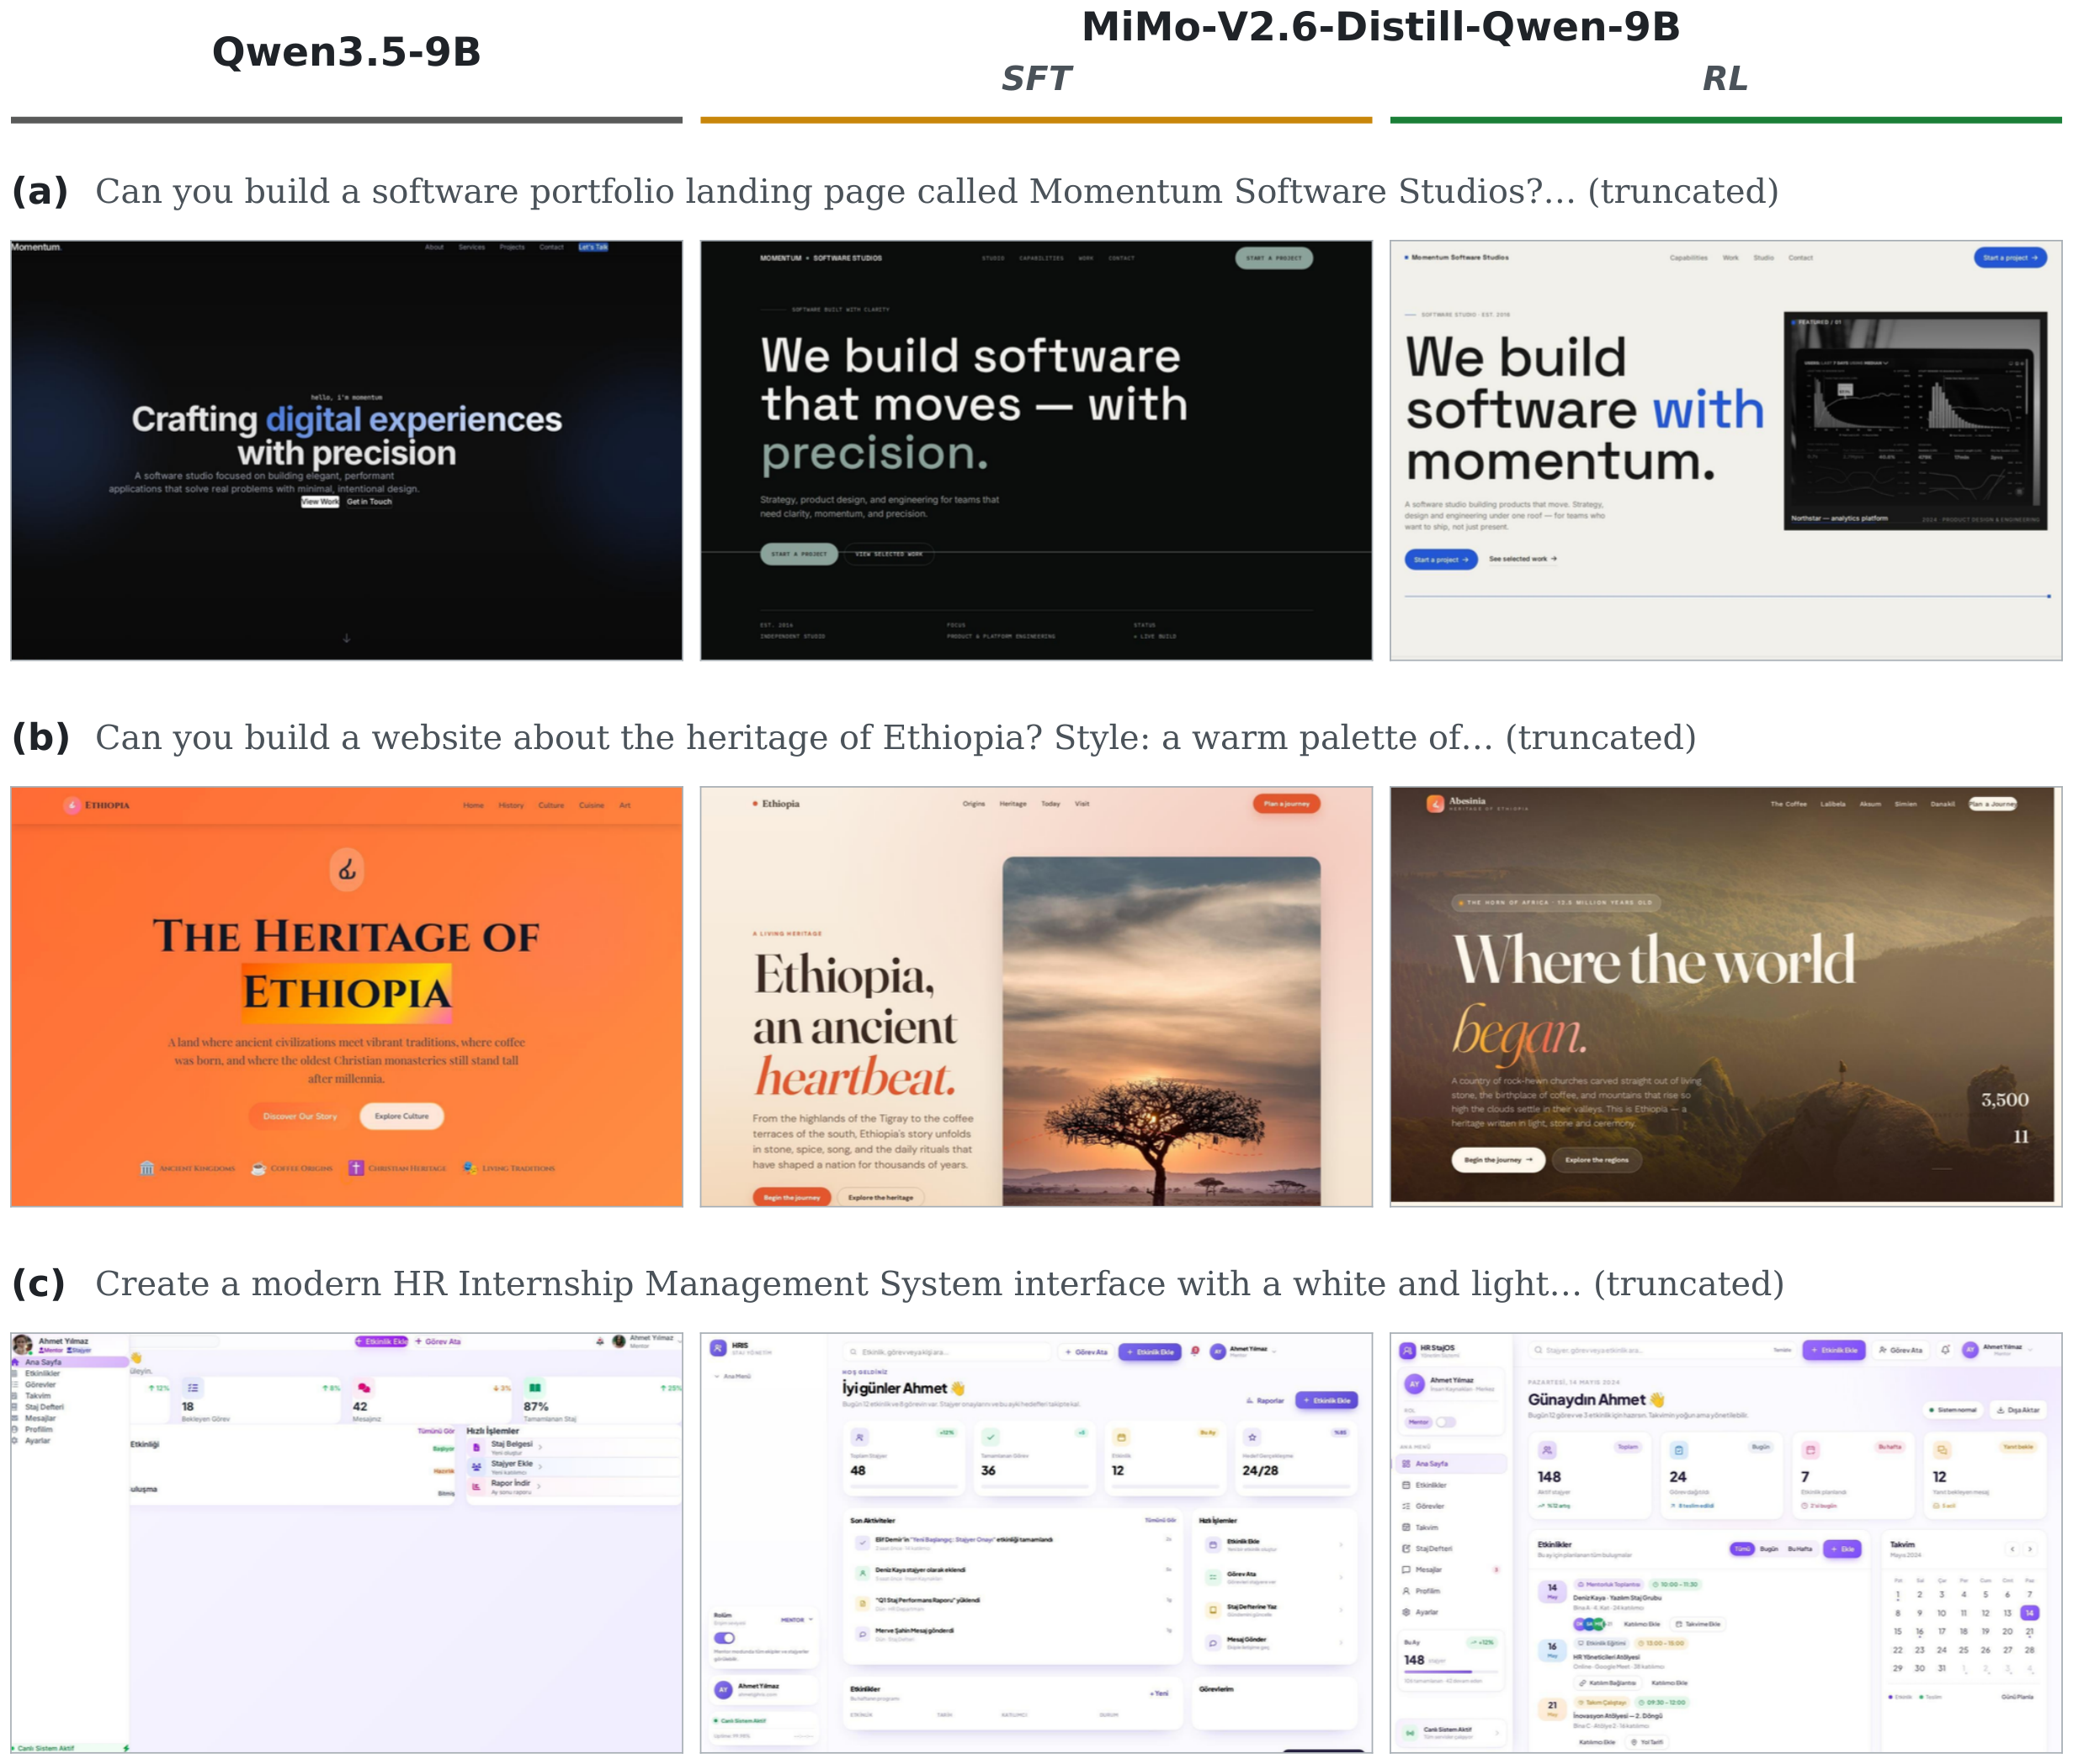
\includegraphics[width=\linewidth]{images_hi/fig17.png}
\caption{由 Qwen3.5-9B、MiMo-V2.6-Distill-Qwen-9B（SFT）和 MiMo-V2.6-Distill-Qwen-9B（RL）生成的网站首屏区域示例。每一行（a--c）展示三个模型对同一提示词的输出。}
\label{fig:17}
\end{figure}

\subsection{References}\label{references}

Artificial Analysis. GDPval-AA v2.1 Leaderboard, 2026. URL
https://artificialanalysis.ai/evalua tions/gdpval-aa. Accessed September
21, 2026.

I. Badertdinov, M. Nekrashevich, A. Shevtsov, and A. Golubev.
Swe-rebench v2: Languageagnostic swe task collection at scale, 2026. URL
https://arxiv.org/abs/2602.23866.

J. Chen, Y. Liang, and Z. Liu. Dflash: Block diffusion for flash
speculative decoding, 2026. URL https://arxiv.org/abs/2602.06036.

Core Team, B. Xiao, B. Xia, B. Yang, B. Gao, B. Shen, C. Zhang, C. He,
C. Lou, F. Luo, et al.~MiMo-V2-Flash technical report, 2026. URL
https://arxiv.org/abs/2601.02780.

X. Deng, J. Da, E. Pan, Y. Y. He, C. Ide, K. Garg, N. Lauffer, A. Park,
N. Pasari, C. Rane, et al.~Swe-bench pro: Can ai agents solve
long-horizon software engineering tasks?, 2025. URL
https://arxiv.org/abs/2509.16941.



F. Gloeckle, B. Y. Idrissi, B. Rozière, D. Lopez-Paz, and G. Synnaeve.
Better \& faster large language models via multi-token prediction. In
Forty-first International Conference on Machine Learning, ICML 2024,
Vienna, Austria, July 21-27, 2024. OpenReview.net, 2024. URL
https://openrevi ew.net/forum?id=pEWAcejiU2.

Z. Han, A. You, H. Wang, K. Luo, G. Yang, W. Shi, M. Chen, S. Zhang, Z.
Lan, C. Deng, et al.~Asyncflow: An asynchronous streaming rl framework
for efficient llm post-training, 2025. URL
https://arxiv.org/abs/2507.01663.

C. He, L. Li, S. Li, H. Lv, L. Kong, Q. Liu, T. Yang, and S. Ren.
Semantic head specialization guides hybrid vit attention for multimodal
llms, 2026. URL https://arxiv.org/abs/2608.28383.

HKUST NLP. Introducing Toolathlon-Verified, June 2026. URL
https://toolathlon.xyz/docs/bl og/toolathlon-verified.

W. Huang and P. Jiang. Deepswe v1.1: a cleaner, more reproducible
benchmark for frontier coding agents, 2026. URL
https://github.com/datacurve-ai/deep-swe.

W. Huang, C. Lee, L. Tng, and S. Ge. Deepswe: Measuring frontier coding
agents on original, long-horizon engineering tasks, 2026. URL
https://arxiv.org/abs/2607.07946.

C. E. Jimenez, J. Yang, A. Wettig, S. Yao, K. Pei, O. Press, and K. R.
Narasimhan. Swe-bench: Can language models resolve real-world github
issues? In The Twelfth International Conference on Learning
Representations, ICLR 2024, Vienna, Austria, May 7-11, 2024.
OpenReview.net, 2024. URL https://openreview.net/forum?id=VTF8yNQM66.

K. Jordan, Y. Jin, V. Boza, J. You, F. Cesista, L. Newhouse, and J.
Bernstein. Muon: An optimizer for hidden layers in neural networks,
2024. URL https://kellerjordan.github.io/posts/muon/.

Kimi Team. Kimi k1.5: Scaling reinforcement learning with llms, 2025.
URL https://arxiv.org/ abs/2501.12599.

H. Lee, J. Liu, D. Kim, Z. Zhang, C. S. Xia, and L. Zhang. Sec-bench
pro: Can language models solve long-horizon software security tasks?,
2026. URL https://arxiv.org/abs/2605.26548.

S. Lee and D. Brumley. Exploitbench: A capability ladder benchmark for
LLM cybersecurity agents, 2026. URL https://arxiv.org/abs/2605.14153.

J. Li, W. Zhao, J. Zhao, W. Zeng, H. Wu, X. Wang, R. Ge, Y. Cao, Y.
Huang, W. Liu, J. Liu, Z. Su, Y. Guo, F. Zhou, L. Zhang, J. Michelini,
X. Wang, X. Yue, S. Zhou, G. Neubig, and J. He. The tool decathlon:
Benchmarking language agents for diverse, realistic, and long-horizon
task execution. In International Conference on Learning Representations,
2026a. URL https://ar xiv.org/abs/2510.25726.

Y. Li, Y. Feng, Z. Xu, Z. Ma, K. Zheng, F. Jiang, X. Sun, R. Shao, Z.
Chen, Y. Huang, X. Han, B. Lee, K. Xu, S. Zeng, H. Hua, X. Zhang, B.
Alomair, R. Krishna, L. Zettlemoyer, P. W. Koh, B. Ramasubramanian, L.
Niu, X. Yue, and R. Poovendran. JobBench: Aligning agent work with human
will, 2026b. URL https://arxiv.org/abs/2605.26329.

B. Liao, H. Dong, C. Monz, X. Xu, L. Dong, and F. Wei. Multi-turn
on-policy distillation with prefix replay, 2026. URL
https://arxiv.org/abs/2607.04763.

K. Lion, F. Hübler, B. Li, A. Orvieto, and N. He. Muown: Row-norm
control for Muon optimization, 2026. URL
https://arxiv.org/abs/2605.10797.



A. Liu, B. Feng, B. Xue, B. Wang, B. Wu, C. Lu, C. Zhao, C. Deng, C.
Zhang, C. Ruan, et al.~Deepseek-v3 technical report, 2024. URL
https://arxiv.org/abs/2412.19437.

A. Liu, A. Mei, B. Lin, B. Xue, B. Wang, B. Xu, B. Wu, B. Zhang, C. Lin,
C. Dong, et al.~Deepseekv3.2: Pushing the frontier of open large
language models, 2025a. URL https://arxiv.org/abs/ 2512.02556.

J. Liu, J. Su, X. Yao, Z. Jiang, G. Lai, Y. Du, Y. Qin, W. Xu, E. Lu, J.
Yan, Y. Chen, H. Zheng, Y. Liu, S. Liu, B. Yin, W. He, H. Zhu, Y. Wang,
J. Wang, M. Dong, Z. Zhang, Y. Kang, H. Zhang, X. Xu, Y. Zhang, Y. Wu,
X. Zhou, and Z. Yang. Muon is scalable for LLM training, 2025b. URL
https://arxiv.org/abs/2502.16982.

W. Ma, H. Zhang, L. Zhao, Y. Song, Y. Wang, Z. Sui, and F. Luo.
Stabilizing moe reinforcement learning by aligning training and
inference routers, 2025. URL https://arxiv.org/abs/2510.1 1370.

W. Ma, J. Wei, L. Zhao, H. Zhang, B. Xiao, L. Li, Q. Yang, B. Gao, Y.
Wang, R. Li, J. Dong, Z. Sui, and F. Luo. Mopd: Multi-teacher on-policy
distillation for capability integration in llm posttraining, 2026. URL
https://arxiv.org/abs/2606.30406.

R. Marten, A. Shaw, I. Bercovich, B. Droste, T. Cerruti, S. Dillmann, R.
Wang, D. Wahdany, A. Hart, K. Krauth, ScaleAI, Snorkel AI, Turing,
gNucleus AI, Boolean AI, N. Carlini, S. Lyu, A. Wei, A. Khatua, B.
Plüster, C. Dwivedi, C. Sutcliffe, Yuming, D. Tivris, D. Wang, H. W. Goh,
H. Xing, H. Lin, I. Salia, J. Seol, J. Bao, J. Ouyang, J. Park, L.
Walsh, L. Kong, M. Ivanov, M. Ubl, M. Liamets, O. Menis, P. Migdal, Q.
Bao, R. Movva, R. Ben Chaim, N. Srinath, S. Bogdanik, S. Yadav, S.
Benjamin, T. Kung, W. Hughes, X. Lan, H. Gupta, S. Mishra, C. Wang, H.
He, J. Tu, K. Montgomery, Z. Tu, A. Naik, D. Mortensen, I. Zhang, Y.
Mathur, E. Liu, K. Singh, M. Yu, S. Feng, V. Gangal, Z. Tao, S. Ruan, J.
Mueller, J. Cabezas, J. Bauer, K. X. Li, R. Zhang, A. Feller, A.
Madayan, L. Chen, B. Feuer, X. Li, B. Li, H. Raj, S. Galler, L. Shi, I.
Segal, K. Buchanan, S. P., R. Desai, A. Schneider, C. Settles, X. Lin,
M. Nezhurina, A. Wang, M. Kowalczyk, J.-X. Zhao, S. Satia, J. Hu, S.
Atef, K. Chen, S. Vance, G. Segato, J. Jitsev, A. Dimakis, M. Merrill,
A. Konwinski, and L. Schmidt. Terminal-Bench, 2026. URL
https://github.com/harbor-framework/terminal-bench/releases/tag/v4.0.0.
Software release, version 4.0.0.

M. A. Merrill, A. G. Shaw, N. Carlini, B. Li, H. Raj, I. Bercovich, L.
Shi, J. Y. Shin, T. Walshe, E. K. Buchanan, J. Shen, G. Ye, H. Lin, J.
Poulos, M. Wang, M. Nezhurina, J. Jitsev, D. Lu, O. M. Mastromichalakis,
Z. Xu, Z. Chen, Y. Liu, R. Zhang, L. L. Chen, A. Kashyap, J.-L. Uslu, J.
Li, J. Wu, M. Yan, S. Bian, V. Sharma, K. Sun, S. Dillmann, A. Anand, A.
Lanpouthakoun, B. Koopah, C. Hu, E. Guha, G. H. S. Dreiman, J. Zhu, K.
Krauth, L. Zhong, N. Muennighoff, R. Amanfu, S. Tan, S. Pimpalgaonkar, T.
Aggarwal, X. Lin, X. Lan, X. Zhao, Y. Liang, Y. Wang, Z. Wang, C. Zhou,
D. Heineman, H. Liu, H. Trivedi, J. Yang, J. Lin, M. Shetty, M. Yang, N.
Omi, N. Raoof, S. Li, T. Y. Zhuo, W. Lin, Y. Dai, Y. Wang, W. Chai, S.
Zhou, D. Wahdany, Z. She, J. Hu, Z. Dong, Y. Zhu, S. Cui, A. Saiyed, A.
Kolbeinsson, J. Hu, C. M. Rytting, R. Marten, Y. Wang, A. Dimakis, A.
Konwinski, and L. Schmidt. Terminal-Bench: Benchmarking agents on hard,
realistic tasks in command line interfaces, 2026. URL
https://arxiv.org/abs/2601.11868.

P. Moritz, R. Nishihara, S. Wang, A. Tumanov, R. Liaw, E. Liang, M.
Elibol, Z. Yang, W. Paul, M. I. Jordan, et al.~Ray: A distributed
framework for emerging \{AI\} applications. In 13th USENIX symposium on
operating systems design and implementation (OSDI 18), pages 561--577,
2018.



K. Opsahl-Ong, A. Singhvi, J. Collins, I. Zhou, C. Wang, A. Baheti, O.
Oertell, J. Portes, S. Havens, E. Elsen, M. Bendersky, M. Zaharia, and
X. Chen. Officeqa pro: An enterprise benchmark for end-to-end grounded
reasoning, 2026. URL https://arxiv.org/abs/2603.08655.

T. Patwardhan, R. Dias, E. Proehl, G. Kim, M. Wang, O. Watkins, S. P.
Fishman, M. Aljubeh, P. Thacker, L. Fauconnet, N. S. Kim, P. Chao, S.
Miserendino, G. Chabot, D. Li, M. Sharman, A. Barr, A. Glaese, and J.
Tworek. GDPval: Evaluating AI model performance on real-world
economically valuable tasks, 2025. URL https://arxiv.org/abs/2510.04374.

PrimeIntellect. Swe-rl: Software engineering tasks for rl, 2026. URL
https://huggingface.co/col lections/PrimeIntellect/swe-rl.

X. Qu, P. Huang, and S. Horvath. Can Muon fine-tune Adam-pretrained
models?, 2026. URL https://arxiv.org/abs/2605.10468.

Qwen Team. Qwen3-next: Towards ultimate training \& inference efficiency.
https://qwen.ai/blog
?id=4074cca80393150c248e508aa62983f9cb7d27cd\&from=research.latest-advancements-list,
September 2025.

I. Shah, A. M. Polloreno, K. Stratos, P. Monk, A. Chaluvaraju, A. Hojel,
A. Ma, A. Thomas, A. Tanwer, D. J. Shah, K. Nguyen, K. Smith, M.
Callahan, M. Pust, M. Parmar, P. Rushton, P. Mazarakis, R. Kapila, S.
Srivastava, S. Singla, T. Romanski, Y. Vanjani, and A. Vaswani.
Practical efficiency of Muon for pretraining, 2025. URL
https://arxiv.org/abs/2505.02222.

Z. Shao, P. Wang, Q. Zhu, R. Xu, J. Song, X. Bi, H. Zhang, M. Zhang, Y.
K. Li, Y. Wu, and D. Guo. Deepseekmath: Pushing the limits of
mathematical reasoning in open language models, 2024. URL
https://arxiv.org/abs/2402.03300.

D. Shepard and R. Salimans. AutomationBench, 2026. URL
https://arxiv.org/abs/2604.18934.

M. Shoeybi, M. Patwary, R. Puri, P. LeGresley, J. Casper, and B.
Catanzaro. Megatron-lm: Training multi-billion parameter language models
using model parallelism, 2019. URL https://arxiv. org/abs/1909.08053.

Y. Sun, X. Han, W. Zhang, Y. Pang, T. Wang, Y. Cao, Y. Huang, C. Duroiu,
H. Zhang, J. Lin, W. Zhang, T. Zeng, Y. Yan, B. Liu, H. Wen, M. Xu, X.
Liu, Z. Chen, W. Shi, A. Dsouza, V. S. Chen, P. Bryant, C. Boettiger, Y.
Rangan, B. Rothenberg, K. Steinfeld, A. Rao, T. Schneider, G.
Yannakakis, L. Zanna, K. Ozbay, I. Sim, T. Zohdi, G. E. Karniadakis, J.
Gallant, T. Head-Gordon, Y. Li, W. Deng, T. Sun, H. Wang, Z. Wang, J.
Xu, C. Y. Liu, Y. Cheng, R. Hu, A. Bacho, S. Cao, Z. Qin, Y. Chen, H.
Fan, H. Liu, L. Zeng, S. M. Bharadwaj, L. Gong, Y. Yang, M. Song, R.
Wang, Z. Zhang, H. Bao, S. Lu, J. Tu, Z. Wang, Z. Zhang, Z. Chen, Y.
Jiang, Z. Li, B. Lyu, C. Ma, P. Xu, B. Zhang, S. Gu, H. Hua, H. Li, W.
Liao, C. Liu, J. Peng, H. Sun, Z. Xu, B. Chen, J. Cheng, Y. Jiang, K.
Kuang, Y. Li, Y. Pan, Z. Rao, A. Schubert, Y. Shen, V. Siu, X. Sun, K.
Zhang, X. Zhang, Y. Zhu, I. S. Chandok, L. Ding, J. Fan, A. Glover, J.
Hu, Y. Hu, W. Huang, Z. Jiang, H. Jin, L. Kim, M. Liu, Y. Liu, A.
Rafiei, X. Shen, K. Sun, S. Sun, T. Sun, E. Wang, Y. Wang, H. Xing, S.
Xu, Y. Xu, Z. Xu, Z. Yan, B. Yuan, R. Zhang, Y. Zhang, Z. Zhao, Liana,
S. B. Antu, H. Bai, C. Bosio, J. Cavanagh, P. Cavazos-Rehg, T. Chen, X.
Chen, Y. Chen, C. Zhu, C. Dai, S. D. Castro, Y. Deng, K. Dhole, J. Ding,
C. Du, Z. Du, H. Fan, R.-Z. Fan, H. Fu, S. Gu, Y. Gu, C. Guo, B. Huang,
B. Huang, R. Jaiswal, Z. Jiang, R. Jin, E. Kasson, X. Lan, J. Lee, D.
Lei, C. Li, D. Li, H. Li, H. Li, J. Li, X. Li, Y. Li, Y. Li, Y. Li, Z.
Li, W. Liang, L. Liao, K. Q. Lin, A. Z. Liu, C. Liu, J. Liu, K. Liu, X.
Liu, P. Lu, W. Lv, Y. Lyu, Q. Mang, K. Montgomery, Y. Nie, R. Ning, J.
Overwiening, X. Pan, L. Paraboschi, C. F. Park, J. Purnomo, S. Rajwal,
S. Rankin, B. Ren, Y. Rong, H. Shang, V. Shaw, F. Shen, J. Shen, M. Shi,
S. Qiu, H. Yao, T. Shi, J. So, V. Susoy, H. Szlyk, H. Wang,



J. Wang, W. Wang, X. Wang, Z. Wang, D. Wong, A. Wu, D. Wu, F. Wu, M. M.
Wu, Y. Wu, Y. Wu, Y. Wu, Q. Wuwu, W. Xiao, Y. Xiong, F. Xu, R. Xu, M.
Yan, B. Yang, J. Yang, S. Yang, X. Yang, Y. Yang, H. Ye, X. Yu, Z. Yu,
C. Zhang, C. Zhang, H. Zhang, H. Zhang, J. Zhang, K. Zhang, S. Zhang, W.
Zhang, W. Zhang, Y. Zhang, Y. Zhang, B. Zhao, Q. Zhao, Y. Zhao, Y.
Zheng, L. Zhou, T. Zhou, S. Zhu, S. Zhu, Y. Zhu, Y. Zhu, J. Zuo, C. Cai,
H. Casademunt, W. Chen, C. Cheng, N. Deng, R. Fu, T. Fu, Y. Han, H. Ren,
Z. He, Q. Jin, L. Li, Y. Li, S. Liu, L. Lu, L. Zhou, S. Mukherjee, Y.
Ouyang, Y. Ren, D. Shi, H. Wu, Z. Wu, H. Yao, Z. Yi, J. Yu, R. Zhan, H.
Zhou, B. Zhu, J. Zhu, A. Yuille, Y. Liu, R. A. Poldrack, J. Li, Z. Li,
M. Tao, J. Huang, W. Shi, C. Spanos, L. Sun, C. Wang, O. Xu, Z. Dong, H.
Gomez, A. Caliskan, A. Emami, H. Hu, Z. Li, L. Liu, M. Niu, Y. Shao, J.
Sun, M. Tolonen, T. Wang, S. Das, Y. Gao, W. Guo, E. J. Schneider, Z.
Lu, Y. Ma, M. Mueller, R. Poovendran, S. Sojoudi, Y. Zhu, and D. Song.
Agents' last exam, 2026. URL https://arxiv.org/abs/2606.05405.

C. Tao, J. Chen, Y. Jiang, K. Kou, S. Wang, R. Wang, X. Li, S. Yang, Y.
Du, J. Dai, Z. Mao, X. Wang, L. Shang, and H. Bai. Swe-lego: Pushing the
limits of supervised fine-tuning for software issue resolving, 2026. URL
https://arxiv.org/abs/2601.01426.

The Microsoft AI Team. MAI-Thinking-1: Building a hill-climbing machine.
Technical report, Microsoft AI, 2026. URL
https://microsoft.ai/pdf/mai-thinking-1.pdf.

A. Vaswani, N. Shazeer, N. Parmar, J. Uszkoreit, L. Jones, A. N. Gomez,
L. Kaiser, and I. Polosukhin. Attention is all you need. In I. Guyon, U.
von Luxburg, S. Bengio, H. M. Wallach, R. Fergus, S. V. N. Vishwanathan,
and R. Garnett, editors, Advances in Neural Information Processing
Systems 30: Annual Conference on Neural Information Processing Systems
2017, December 4-9, 2017, Long Beach, CA, USA, pages 5998--6008, 2017.
URL https://proceedings.neurips.
cc/paper/2017/hash/3f5ee243547dee91fbd053c1c4a845aa-Abstract.html.

vLLM Project. Humming. https://github.com/vllm-project/humming/releases/tag/v0.1.15,
September 2026. Version 0.1.15, GitHub repository, commit
a74973b5079e42ef861720b62f847ce9d33447f5; accessed 2026-09-19.

Z. Wang, T. Shi, J. He, M. Cai, J. Zhang, and D. Song. Cybergym:
Evaluating AI agents' cybersecurity capabilities with real-world
vulnerabilities at scale, 2025. URL https://arxiv.org/abs/ 2506.02548.

Z. Wang, N. Schiller, H. Li, S. S. Narayana, M. Nasr, N. Carlini, X. Qi,
E. Wallace, E. Bursztein, L. Invernizzi, K. Thomas, Y. Shoshitaishvili,
W. Guo, J. He, T. Holz, and D. Song. Exploitgym: Can AI agents turn
security vulnerabilities into real attacks?, 2026. URL
https://arxiv.org/ab s/2605.11086.

B. Xia, B. Shen, D. Zhu, D. Zhang, G. Wang, H. Zhang, H. Liu, J. Xiao,
J. Dong, L. Zhao, et al.~Mimo: Unlocking the reasoning potential of
language model--from pretraining to posttraining, 2025. URL
https://arxiv.org/abs/2505.07608.

L. Xiaomi. Mimo-audio: Audio language models are few-shot learners,
2025. URL https://arxiv. org/abs/2512.23808.

T. Xie, D. Zhang, J. Chen, X. Li, S. Zhao, R. Cao, T. J. Hua, Z. Cheng,
D. Shin, F. Lei, Y. Liu, Y. Xu, S. Zhou, S. Savarese, C. Xiong, V.
Zhong, and T. Yu. Osworld: Benchmarking multimodal agents for open-ended
tasks in real computer environments. In A. Globersons, L. Mackey, D.
Belgrave, A. Fan, U. Paquet, J. M. Tomczak, and C. Zhang, editors,
Advances in Neural Information Processing Systems 37: Annual Conference
on Neural Information Processing Systems 2024, NeurIPS 2024, Vancouver,
BC, Canada, December 10 - 15, 2024, 2024. doi: 10.52202/07901



7-1650. URL
http://papers.nips.cc/paper\_files/paper/2024/hash/5d413e48f84dc61244b6be5
50f1cd8f5-Abstract-Datasets\_and\_Benchmarks\_Track.html.

XLANG Lab. Introducing OSWorld-Verified, July 2025. URL
https://xlang.ai/blog/osworld-verif ied.

W. Xu, R. Han, Z. Wang, L. T. Le, D. Madeka, L. Li, W. Y. Wang, R.
Agarwal, C. Lee, and T. Pfister. Speculative knowledge distillation:
Bridging the teacher-student gap through interleaved sampling. In The
Thirteenth International Conference on Learning Representations, ICLR
2025, Singapore, April 24-28, 2025. OpenReview.net, 2025. URL
https://openreview.net/forum?i d=EgJhwYR2tB.

J. Yang, K. Lieret, J. Ma, P. Thakkar, D. Pedchenko, S. Sootla, E.
McMilin, P. Yin, R. Hou, G. Synnaeve, D. Yang, and O. Press.
Programbench: Can language models rebuild programs from scratch?, 2026a.
URL https://arxiv.org/abs/2605.03546.

S. Yang, C. Tao, J. Chen, T. Yu, R. Wang, Y. Jiang, Y. Du, W. Xu, J.
Xiong, T. Wu, L. Shang, X. Li, N. Wong, and H. Bai. What makes
interaction trajectories effective for training terminal agents?, 2026b.
URL https://arxiv.org/abs/2606.03461.

B. Ye, L. Li, S. Li, Z. Yue, L. Zhang, H. Lv, Y. Liu, W. Ma, H. Tian, R.
Li, J. Dong, Y. Zhao, X. Deng, H. Zhang, L. Zhao, Q. Liu, L. Kong, T.
Yang, and F. Luo. CodeMidas: Scaling agentic coding rl environments from
code itself, 2026. URL https://arxiv.org/abs/2609.22068.

Q. Yu, Z. Zhang, R. Zhu, Y. Yuan, X. Zuo, Y. Yue, W. Dai, T. Fan, G.
Liu, J. Liu, L. Liu, X. Liu, H. Lin, Z. Lin, B. Ma, G. Sheng, Y. Tong,
C. Zhang, M. Zhang, R. Zhang, W. Zhang, H. Zhu, J. Zhu, J. Chen, J.
Chen, C. Wang, H. Yu, Y. Song, X. Wei, H. Zhou, J. Liu, W. Ma, Y. Zhang,
L. Yan, Y. Wu, and M. Wang. DAPO: an open-source LLM reinforcement
learning system at scale. In D. Belgrave, C. Zhang, L. N. Montoya, H.
Lin, R. Pascanu, P. Koniusz, M. Ghassemi, N. Chen, I. V. M. Ruíz, and A.
Loaiza-Bonilla, editors, Advances in Neural Information Processing
Systems 38: Annual Conference on Neural Information Processing Systems
2025, NeurIPS 2025, San Diego, CA, USA, December 2-7, 2025 / Mexico
City, Mexico, November 30 - December 5, 2025, 2025. URL
http://papers.nips.cc/paper\_files/paper/2025/hash/a4277
440d50f1f15d2cb4c14f7e0c0d2-Abstract-Conference.html.

Z. Yue, Z. Lin, Y. Song, W. Wang, S. Ren, S. Gu, S. Li, P. Li, L. Zhao,
L. Li, et al.~Mimo-vl technical report, 2025. URL
https://arxiv.org/abs/2506.03569.

D. Zan, Z. Huang, W. Liu, H. Chen, S. Xin, L. Zhang, Q. Liu, A. Li, L.
Chen, X. Zhong, S. Liu, Y. Xiao, L. Chen, Y. Zhang, J. Su, T. Liu, R.
Long, M. Ding, and L. Xiang. Multi-swebench: A multilingual benchmark
for issue resolving. In D. Belgrave, C. Zhang, L. N. Montoya, H. Lin, R.
Pascanu, P. Koniusz, M. Ghassemi, N. Chen, I. V. M. Ruíz, and A.
Loaiza-Bonilla, editors, Advances in Neural Information Processing
Systems 38: Annual Conference on Neural Information Processing Systems
2025, NeurIPS 2025, San Diego, CA, USA, December 2-7, 2025 / Mexico
City, Mexico, November 30 - December 5, 2025, 2025. URL http:
//papers.nips.cc/paper\_files/paper/2025/hash/5afa9cb1e917b898ad418216dc726fbd-A
bstract-Datasets\_and\_Benchmarks\_Track.html.

J. Zhao, G. Chen, F. Meng, M. Li, J. Chen, H. Xu, Y. Sun, X. Zhao, R.
Song, Y. Zhang, P. Wang, C. Chen, J. Wen, and K. Jia. Immersion in the
github universe: Scaling coding agents to mastery, 2026. URL
https://arxiv.org/abs/2602.09892.



L. Zheng, L. Yin, Z. Xie, C. Sun, J. Huang, C. H. Yu, S. Cao, C.
Kozyrakis, I. Stoica, J. E. Gonzalez, C. W. Barrett, and Y. Sheng.
Sglang: Efficient execution of structured language model programs. In A.
Globersons, L. Mackey, D. Belgrave, A. Fan, U. Paquet, J. M. Tomczak,
and C. Zhang, editors, Advances in Neural Information Processing Systems
37: Annual Conference on Neural Information Processing Systems 2024,
NeurIPS 2024, Vancouver, BC, Canada, December 10 - 15, 2024, 2024. URL
http://papers.nips.cc/paper\_files/paper/2024/hash/724be4472168f31
ba1c9ac630f15dec8-Abstract-Conference.html.
